\chapter{Resultados}
\label{Resultados}

O Plano Semestral de Trabalho dos Docentes do \ac{IFG} é um documento que precisa ser impreterivelmente confeccionado e entregue à Chefia do Departamento de Áreas Acadêmicas dos \textit{campi}.
O documento é normatizado nos termos da Resolução 09 de 1º de Novembro de 2011 do \ac{IFG}~\citep{resolucao}.
Este Trabalho de Conclusão de Curso, conforme definido no objetivo, almejou construir uma solução \textit{user-friendly} e independente de sistema operacional para a elaboração do Plano Semestral de Trabalho nos termos da Resolução 09 de 1º de Novembro de 2011 do \ac{IFG}.

A partir da prototipação como metodologia de desenvolvimento de software, utilizando tecnologias de desenvolvimento \textit{Web}, um banco de dados \ac{NoSQL} baseado em documentos e SCRUM como metodologia de gerenciamento do projeto, foi construída uma aplicação \textit{web} para o preenchimento do documento ``Plano Semestral de Trabalho Docente'' de acordo com a Resolução nº 09 de 1º de Novembro de 2011~\citep{resolucao}.

A aplicação funciona em qualquer browser e se ajusta de forma automática ao tamanho da tela do usuário, o que a torna independente de sistema operacional.
Além disso, a usabilidade da aplicação foi ajustada atualizando o layout conforme solicitações dos \textit{stakeholders} ao final de cada \textit{Sprint}.
Tais ajustes atualizaram tanto o protótipo inicial, quanto as regras de negócio.

Os resultados são apresentados neste texto sob a forma de figuras das telas do sistema, o qual está em sua versão inicial (1.0) disponível para implantação por parte do \textit{campus} Formosa do \ac{IFG}.

A Figura \ref{fig:result01} mostra a tela inicial do sistema no qual foi adicionado um botão de início do \nameref{fig:prot01}, para melhorar a navegação.
A Figura \ref{fig:result02} mostra a tela de identificação do usuário, o campo \textit{e-mail} foi adicionado do \nameref{fig:prot02}, para ser possível enviar \textit{e-mail} para o usuário com o link de busca do formulário.
A Figura \ref{fig:result03} mostra a tela de cadastro da qualificação do docente.
A Figura \ref{fig:result04} mostra a tela de cadastro de atividades de ensino.
A Figura \ref{fig:result05} mostra a tela de cadastro de atividades de pesquisa.
A Figura \ref{fig:result06} mostra a tela de cadastro de atividades de extensão.
A Figura \ref{fig:result07} mostra a tela de cadastro de atividades de produção acadêmica e cultural.
A Figura \ref{fig:result08} mostra a tela de cadastro de atividades de qualificação, que não havia sido prototipada.
A Figura \ref{fig:result09} mostra a tela de cadastro de atividades de representação.
A Figura \ref{fig:result10} mostra a tela de finalização do formulário.
A Figura \ref{fig:result11} mostra a mensagem de que o formulário foi salvo com sucesso.
A Figura \ref{fig:result12} mostra a tela de busca do formulário.
A figura \ref{fig:email} mostra o \textit{e-mail} que é enviado ao usuário com o link de acesso do formulário preenchido.


\begin{figure}[htb]
    \centering
    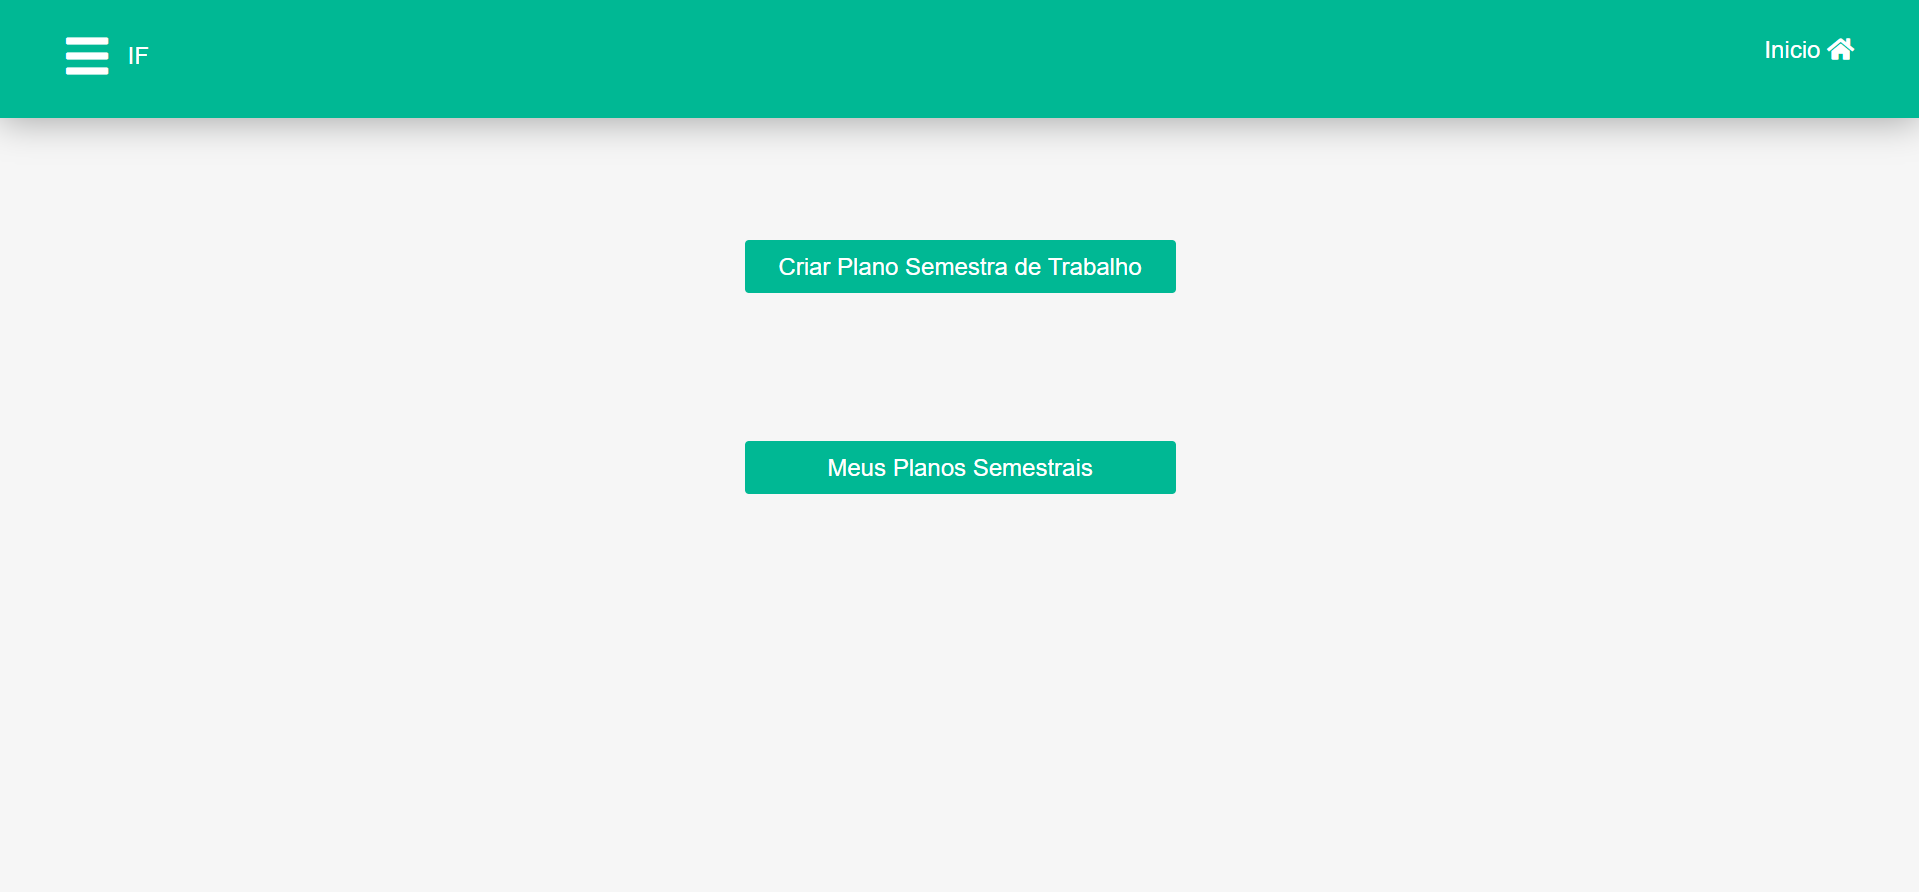
\includegraphics[width=.99\textwidth]{img/pagina_inicial.PNG}
    \caption[Resultado 01: Tela inicial]{Resultado 01: Tela inicial.}
    \label{fig:result01}
\end{figure}

\begin{figure}[htb]
    \centering
    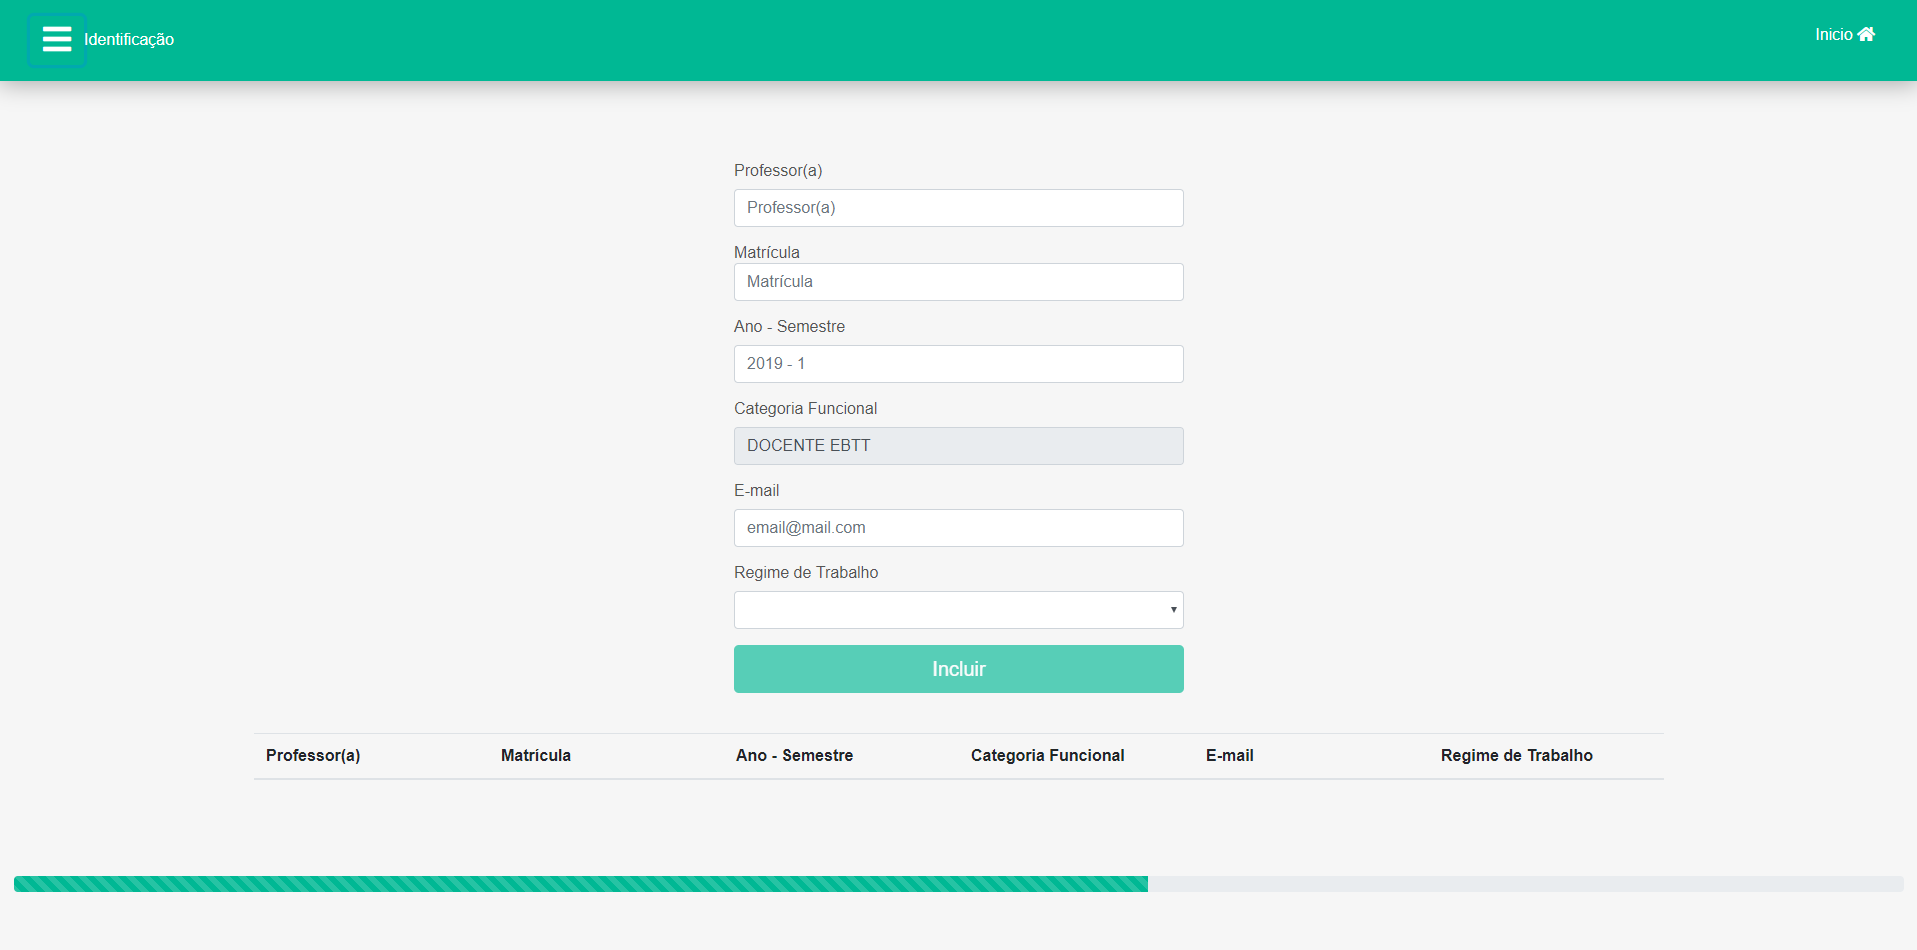
\includegraphics[width=.99\textwidth]{img/pagina_identificacao.PNG}
    \caption[Resultado 02: Tela de Identificação]{Resultado 02: Tela de Identificação.}
    \label{fig:result02}
\end{figure}

\begin{figure}[htb]
    \centering
    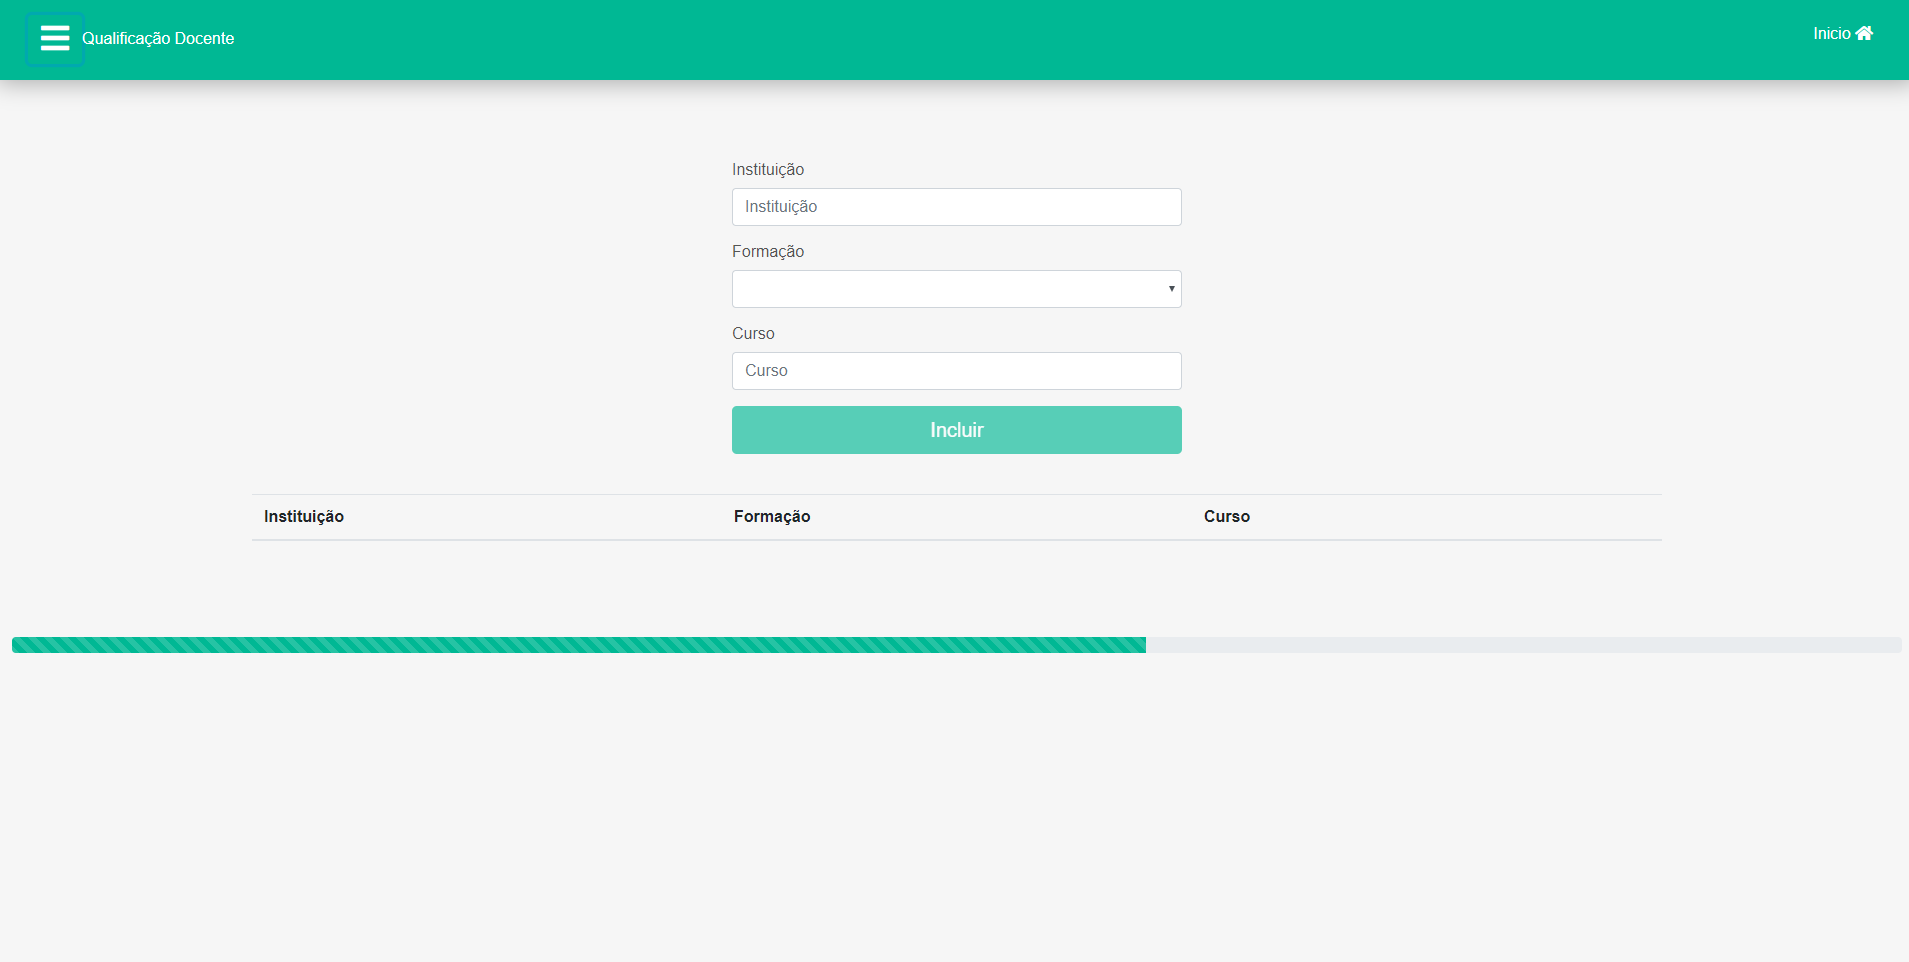
\includegraphics[width=.8\textwidth]{img/pagina_qualificacao_docente.PNG}
    \caption[Resultado 03: Tela de Qualificação do Docente]{Resultado 03: Tela de Qualificação do Docente.}
    \label{fig:result03}
\end{figure}

\begin{figure}[htb]
    \centering
    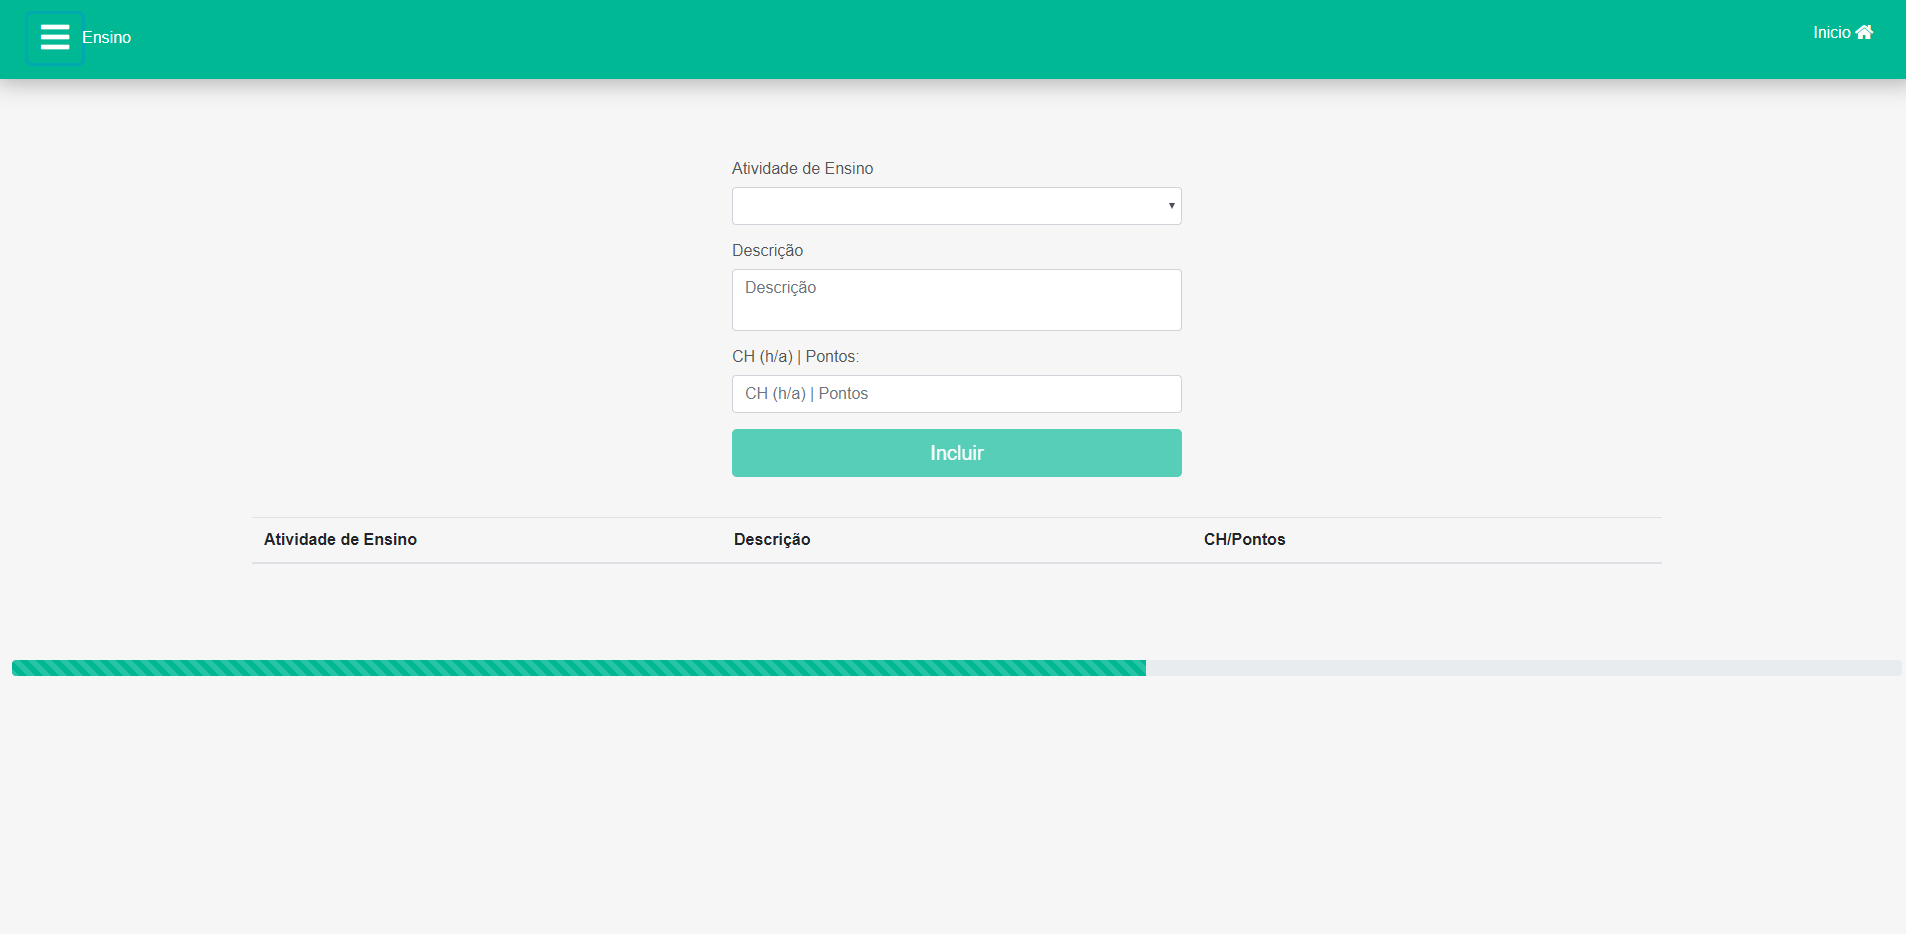
\includegraphics[width=.8\textwidth]{img/pagina_ensino.PNG}
    \caption[Resultado 04: Tela de Atividades de Ensino]{Resultado 04: Tela de Atividades de Ensino.}
    \label{fig:result04}
\end{figure}

\begin{figure}[htb]
    \centering
    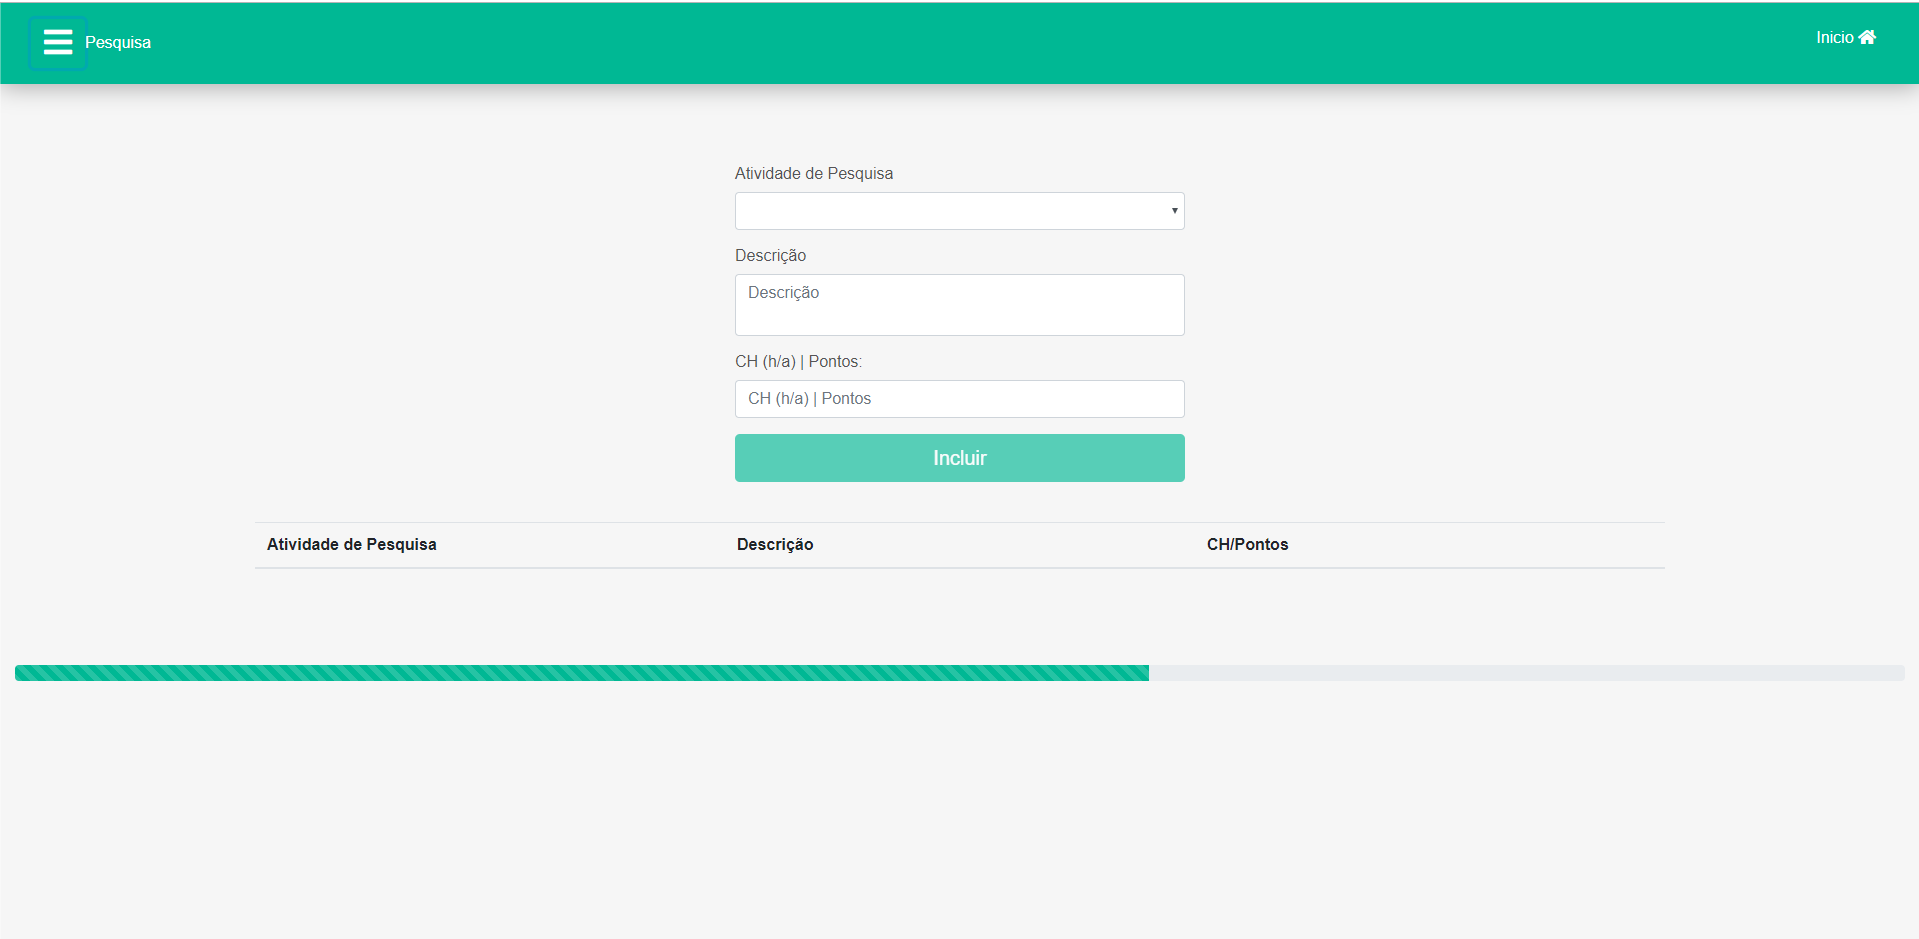
\includegraphics[width=.8\textwidth]{img/pagina_pesquisa.PNG}
    \caption[Resultado 05: Tela de Atividades de Pesquisa]{Resultado 05: Tela de Atividades de Pesquisa.}
    \label{fig:result05}
\end{figure}

\begin{figure}[htb]
    \centering
    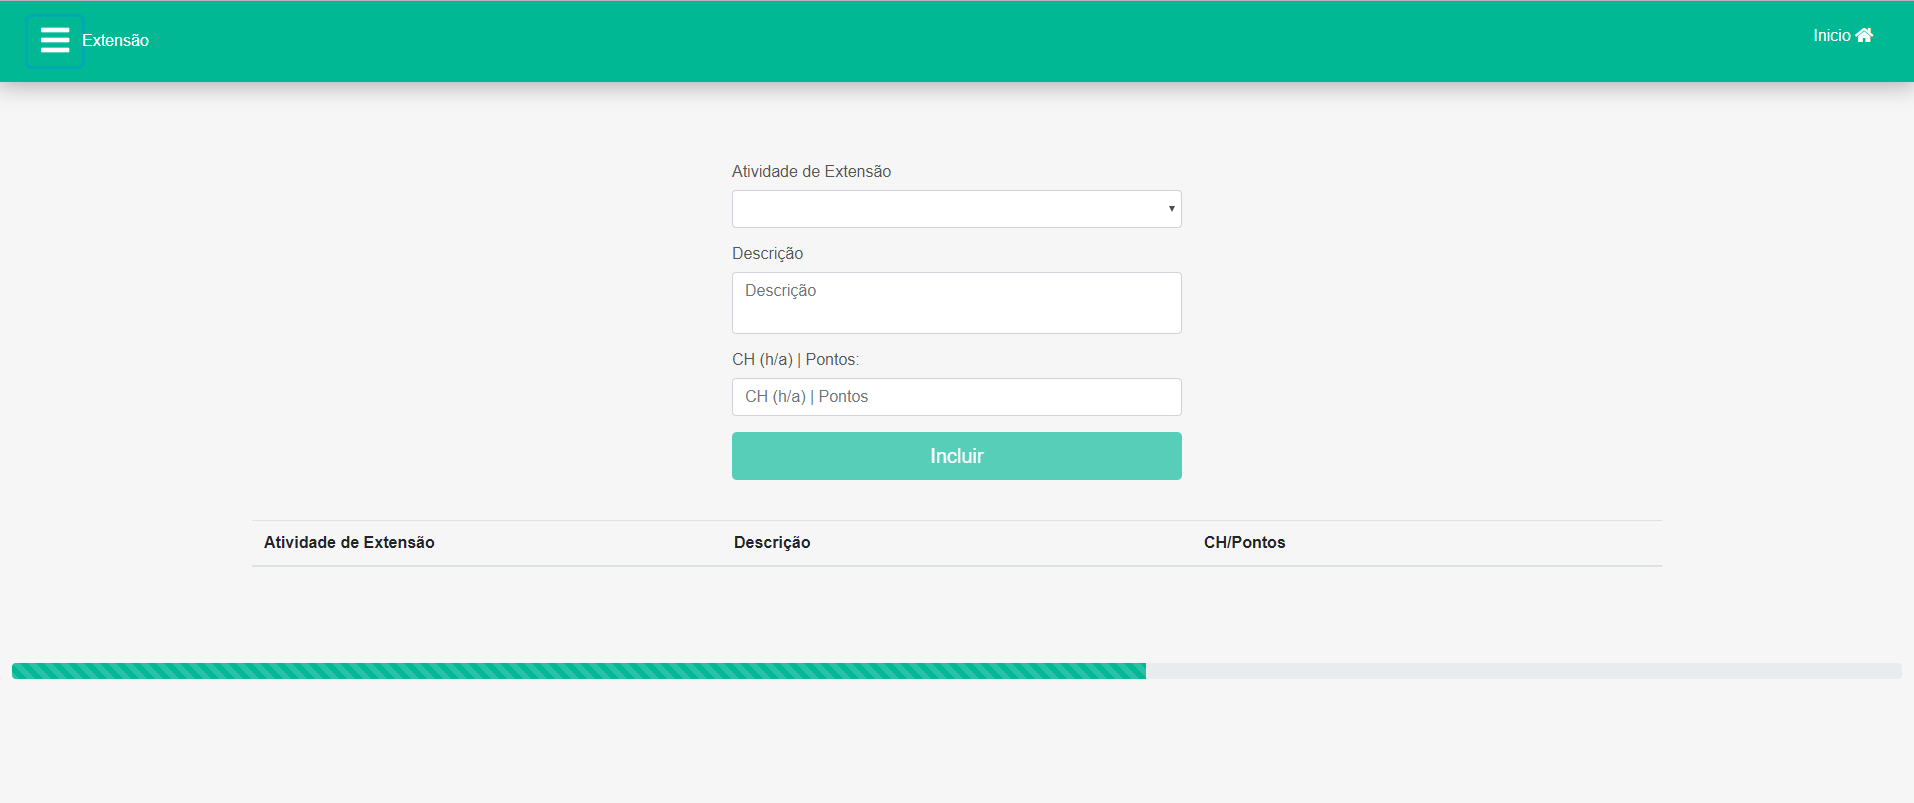
\includegraphics[width=.8\textwidth]{img/pagina_extensao.PNG}
    \caption[Resultado 06: Tela de Atividades de Extensão]{Resultado 06: Tela de Atividades de Extensão.}
    \label{fig:result06}
\end{figure}

\begin{figure}[htb]
    \centering
    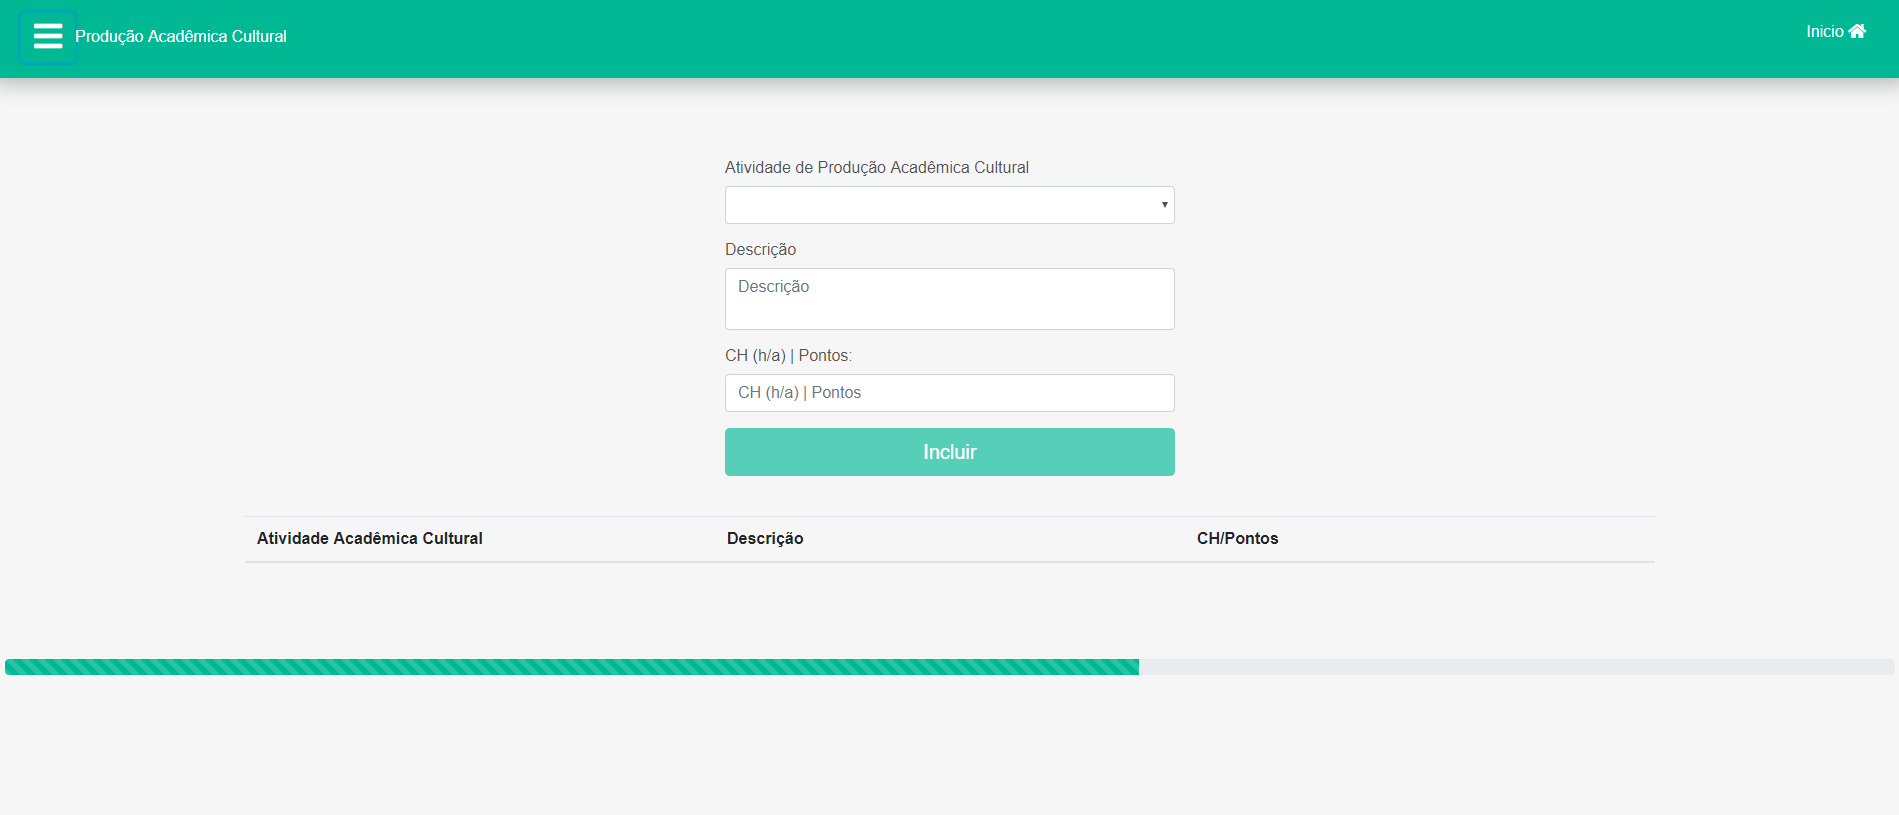
\includegraphics[width=.8\textwidth]{img/pagina_producao.PNG}
    \caption[Resultado 07: Tela de Atividades de Produção Acadêmica]{Resultado 07: Tela de Atividades de Produção Acadêmica.}
    \label{fig:result07}
\end{figure}

\begin{figure}[htb]
    \centering
    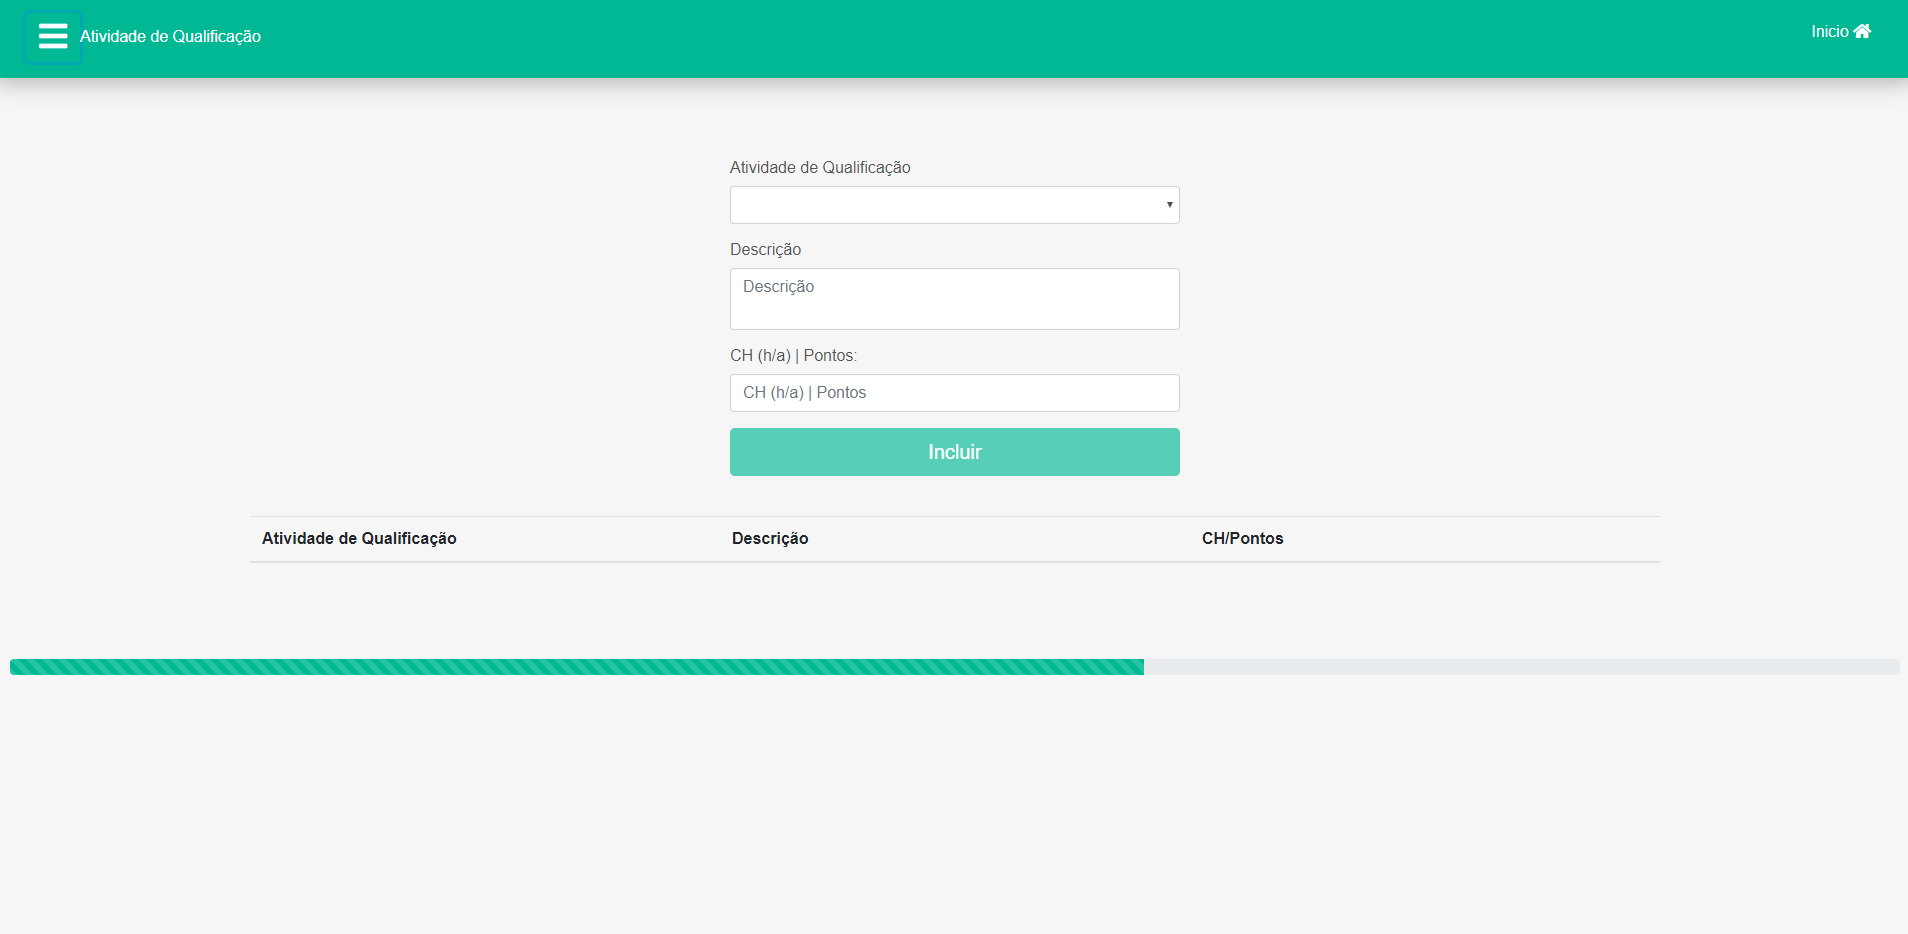
\includegraphics[width=.8\textwidth]{img/pagina_at_qualificacao.PNG}
    \caption[Resultado 08: Tela de Atividades Qualificação]{Resultado 08: Tela de Atividades Qualificação.}
    \label{fig:result08}
\end{figure}

\begin{figure}[htb]
    \centering
    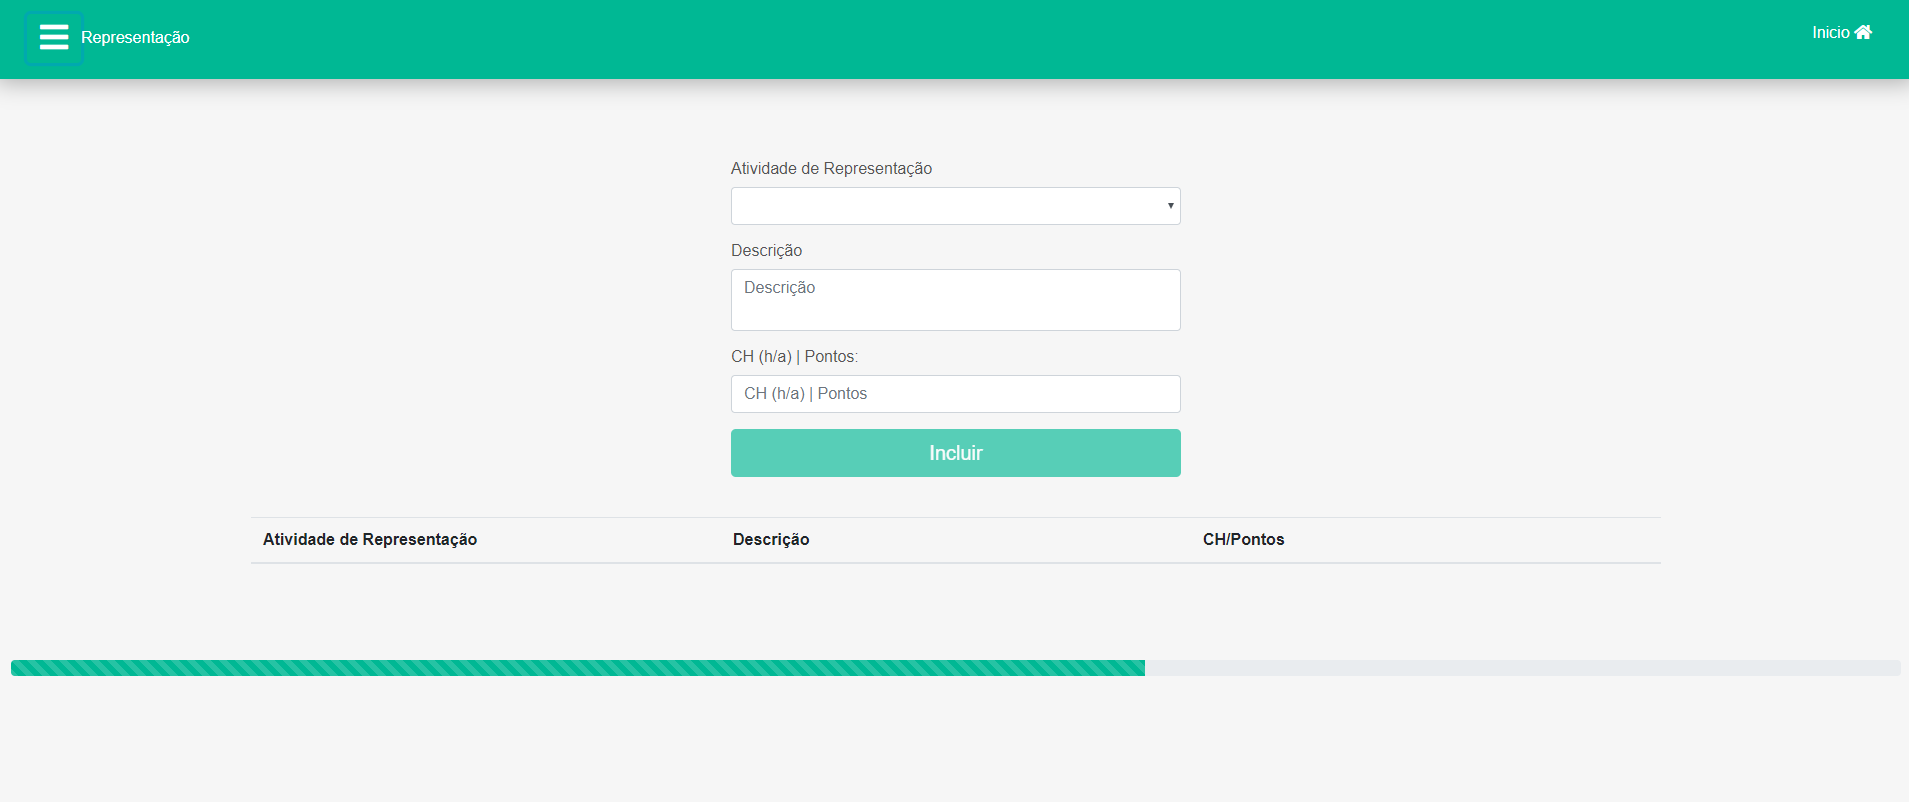
\includegraphics[width=.8\textwidth]{img/pagina_representacao.PNG}
    \caption[Resultado 09: Tela de Atividades Representação]{Resultado 09: Tela de Atividades Representação.}
    \label{fig:result09}
\end{figure}

\begin{figure}[htb]
    \centering
    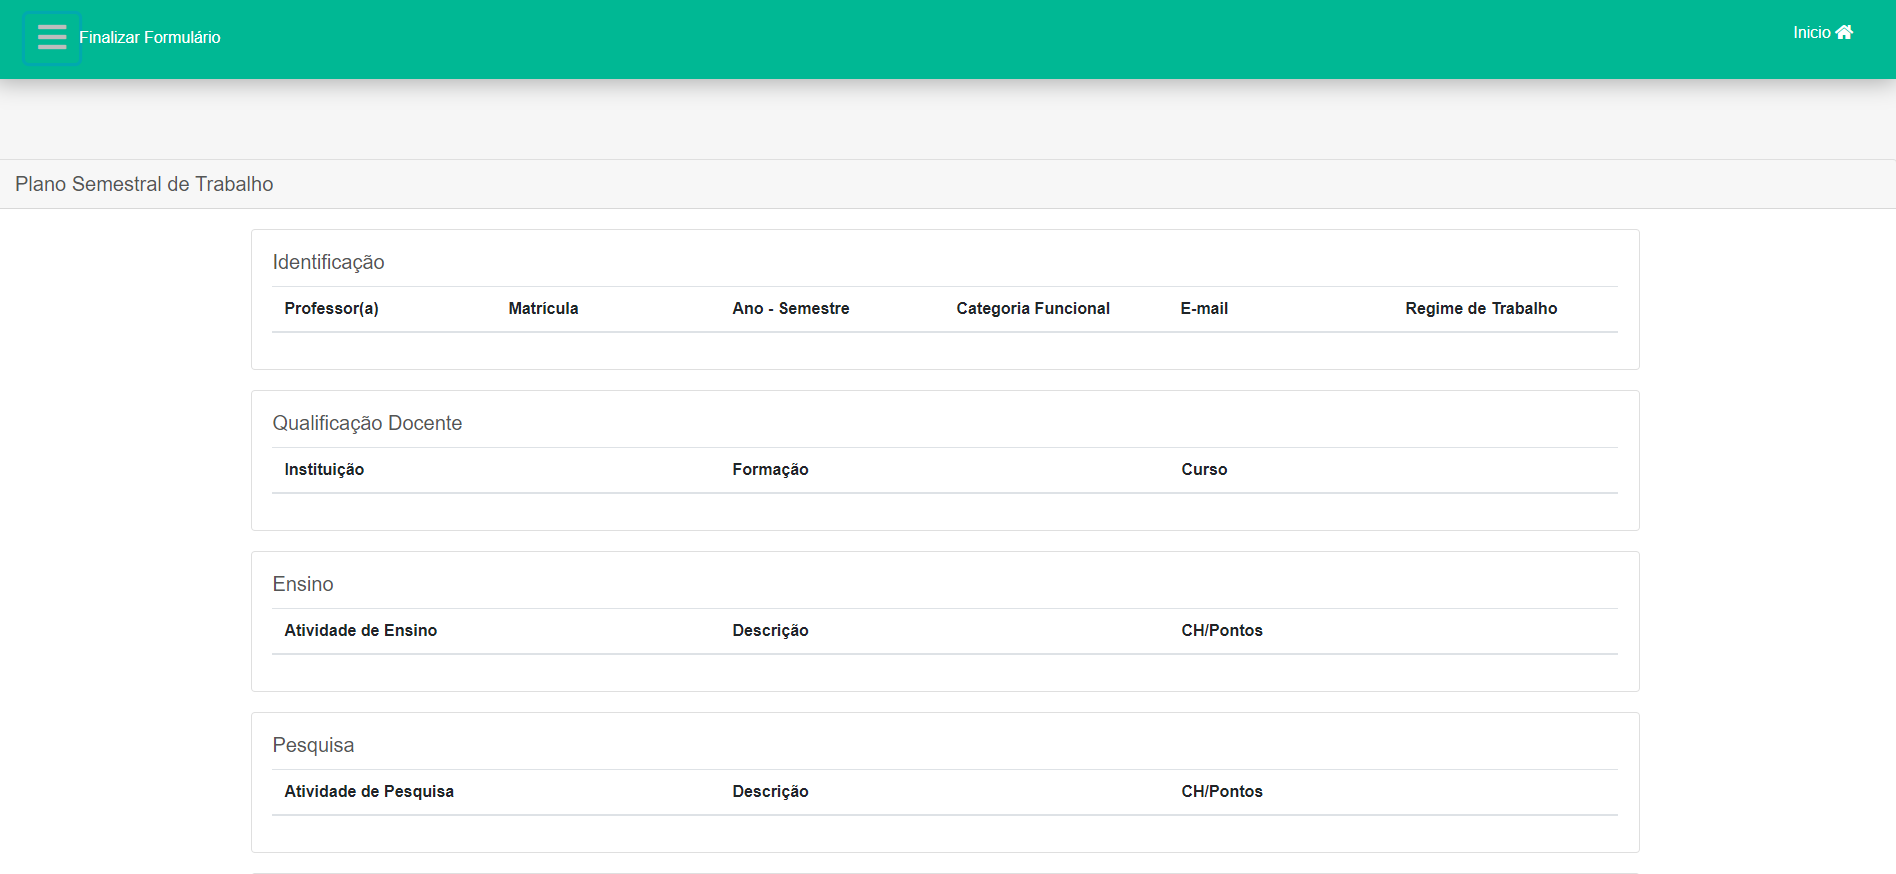
\includegraphics[width=.8\textwidth]{img/pagina_finalizar.PNG}
    \caption[Resultado 10: Tela de Finalização do Formulário]{Resultado 10: Tela de Finalização do Formulário.}
    \label{fig:result10}
\end{figure}

\begin{figure}[htb]
    \centering
    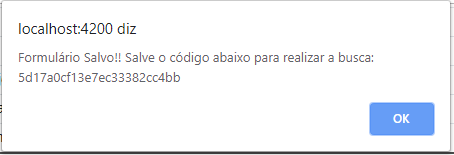
\includegraphics[width=.8\textwidth]{img/alert_salvar.PNG}
    \caption[Resultado 11: Tela de Mensagem de Formulário Salvo]{Resultado 11: Tela de Mensagem de Formulário Salvo.}
    \label{fig:result11}
\end{figure}

\begin{figure}[htb]
    \centering
    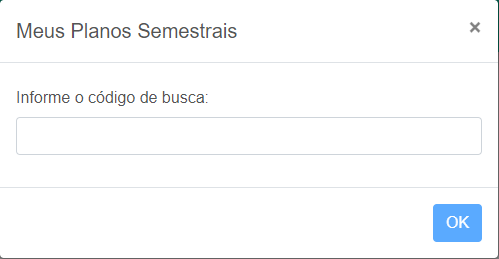
\includegraphics[width=.8\textwidth]{img/pagina_busca.PNG}
    \caption[Resultado 12: Tela de Busca do Formulário Salvo]{Resultado 12: Tela de Busca do Formulário Salvo.}
    \label{fig:result12}
\end{figure}


\begin{figure}[htb]
    \centering
    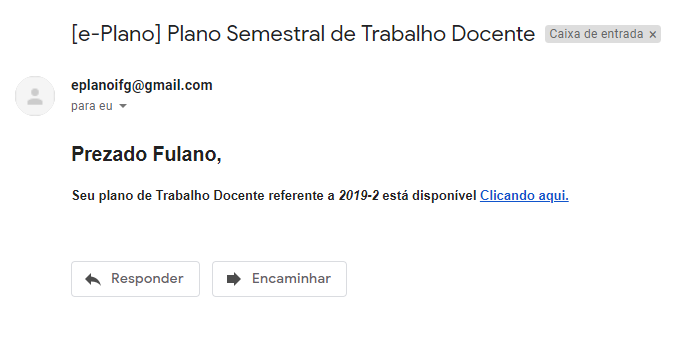
\includegraphics[width=0.8\textwidth]{img/email2.PNG}
    \caption[Resultado 13: \textit{E-mail}]{Resultado 13: \textit{E-mail enviado pelo sistema para acesso ao Plano Semestral de Trabalho Docente}.}
    \label{fig:email}
\end{figure}
